%Siehe tolle Daten in Tab. \ref{tab:impl:data}.
%
%%\begin{table}
%%    \centering
%%    \begin{tabular}{|lcc|}
%%    \hline
%%              & \textbf{Regular Customers} & \textbf{Random Customers} \\ \hline
%%    Age       & 20-40                      & \textgreater{}60          \\ \hline
%%    Education & university                 & high school               \\ \hline
%%    \end{tabular}
%%    \caption{Ein paar tabellarische Daten}
%%    \label{tab:impl:data}
%%\end{table}
%%
%%\begin{figure}
%%    \centering
%%    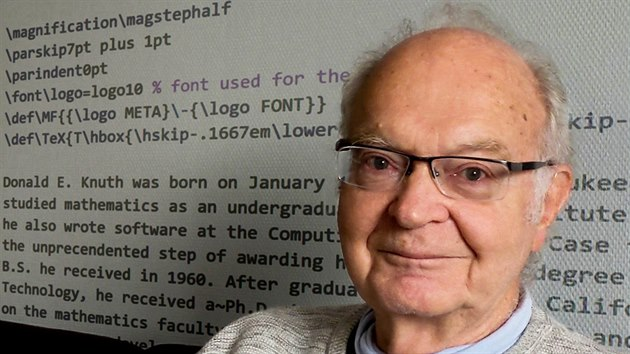
\includegraphics[scale=0.5]{pics/knuthi.jpg}
%%    \caption{Don Knuth -- CS Allfather}
%%    \label{fig:impl:knuth}
%%\end{figure}
%%
%%Siehe und staune in Abb. \ref{fig:impl:knuth}.
%%\lipsum[6-9]
%%Dann betrachte den Code in Listing \ref{lst:impl:foo}.
%%
%%\begin{lstlisting}[language=Python,caption=Some code,label=lst:impl:foo]
%%# Program to find the sum of all numbers stored in a list (the not-Pythonic-way)
%%
%%# List of numbers
%%numbers = [6, 5, 3, 8, 4, 2, 5, 4, 11]
%%
%%# variable to store the sum
%%sum = 0
%%
%%# iterate over the list
%%for val in numbers:
%%    sum = sum+val
%%
%%print("The sum is", sum)
%\end{lstlisting}

\section{Aufbau}\label{sec:assembly}

Folgend werden alle Gegenstände und Geräte für den Aufbau in Abbildung~\ref{fig:assembly} benannt.

\begin{figure}
    \centering
    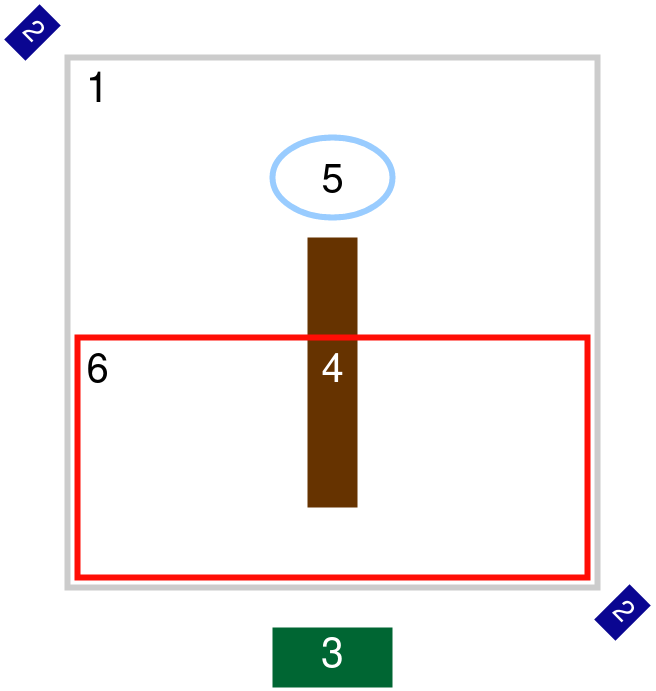
\includegraphics[scale=0.5]{pics/assemlbly}
    \caption{Aufbau}
    \label{fig:assembly}
\end{figure}

\begin{enumerate}
    \item VR Raum
    \item Lichtboxen~\ref{sec:lighthouse}
    \item Bildschirm
    \item Balken
    \item Startposition
    \item Abgrund
\end{enumerate}

\subsection{Erklärung}\label{subsec:description}

Der Spieler bei der Startposition starten und dann Richtung Abgrund dem Balken entlang balancieren.
Die Lichtboxen müssen diagonal positioniert werden wie bereits beschrieben in dem Abschnitt~\ref{sec:lighthouse}.
Der Balken sollte ca in der Mitte sein.

Leichte Versetzungen sidn nicht tragisch. Hierbei geht es nur darum, dass der Balken nicht aus dem VR Raum
rausschaut, da das Tracking dort abbricht. Die position des Bildschirmes ist nicht wichtig.
Hierbei geht es nur um das Steam VR Setup welches bereits in dem Kapitel Steam besprochen worden ist.

\section{Code}\label{sec:code}
\subsection{Ganzkörper-Tracking}\label{sec:full-body-tracking}
\subsection{Beam Calibration}\label{subsec:beam-calibration}
\subsection{Schwerkraft}\label{subsec:gravity}
\subsection{Verkehrssystem}\label{subsec:traffic-system}


\section{3d Welt}\label{sec:3d-world}
Jedes Spiel braucht heutzutage eine Spielwelt, hierbei ist es egal ob es sich um eine 3D oder 2D Applikation handelt.
Unter dem Begriff Spielwelt fällt die Umgebung in welcher sich der Spieler befindet.
Es gibt hierbei so gut wie keine Einschränkungen in der Kreativität, egal ob die digitale Welt nun ein riesiger Ring, der im Weltall schwebt,
oder eine Ansammlung an verschiedenen Planeten ist.
~\cite{GamesRadar_HaloRing_2022}


%% this image and the next are not working. see issue #1

\begin{figure}
    \centering
    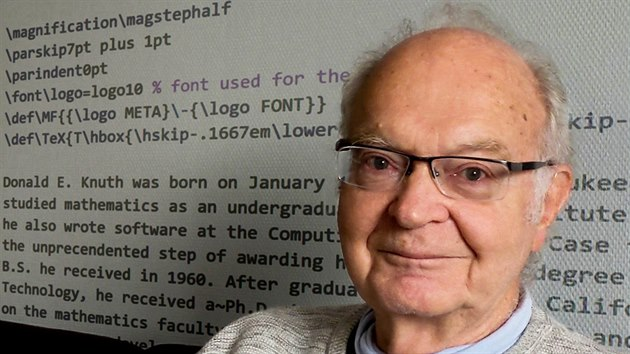
\includegraphics{pics/knuthi}
    \caption{3D Welt - Halo}
    \label{fig:3d_environment_halo}
\end{figure}


%% Grafik für Destiny 2 Locations noch einbinden (Seite für Quelle lädt grade nicht Bungie.net)

\begin{figure}
    \centering
    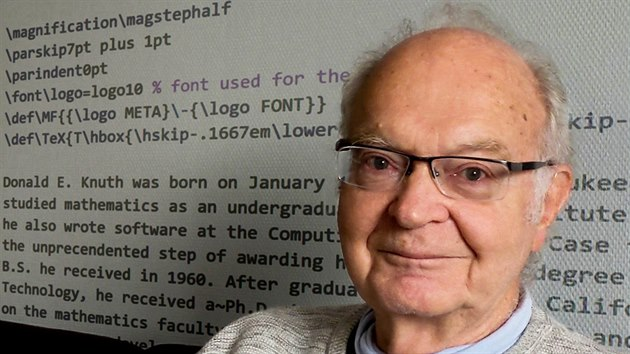
\includegraphics{pics/knuthi}
    \caption{3D Welt - Destiny 2}
    \label{fig:3d_environment_destiny2}
\end{figure}

Spielehersteller bauen die Spielwelten so auf, wie es am besten zu der Vision den Spieles passt.
Gleichzeitig wird darauf geschaut, dass sich die Umgebung nicht langweilig oder leer anfühlt.
Hierfür wird Environmental Storytelling verwendet, darunter versteht man das platzieren von Gegenständen und Objekten
welche dem Spieler eine kleine Geschichte erzählen.
Das passiert jedoch nicht über Sprache sondern einfach nur über die Platzierung und das Aussehen.
Ein Beispiel hierfür w\"are ein das Bild von Cayde-6 (ein Charakter aus Destiny 2), welches in einem Restaurant platziert wurde.
~\cite{GameDeveloper_2022}

\begin {figure}
    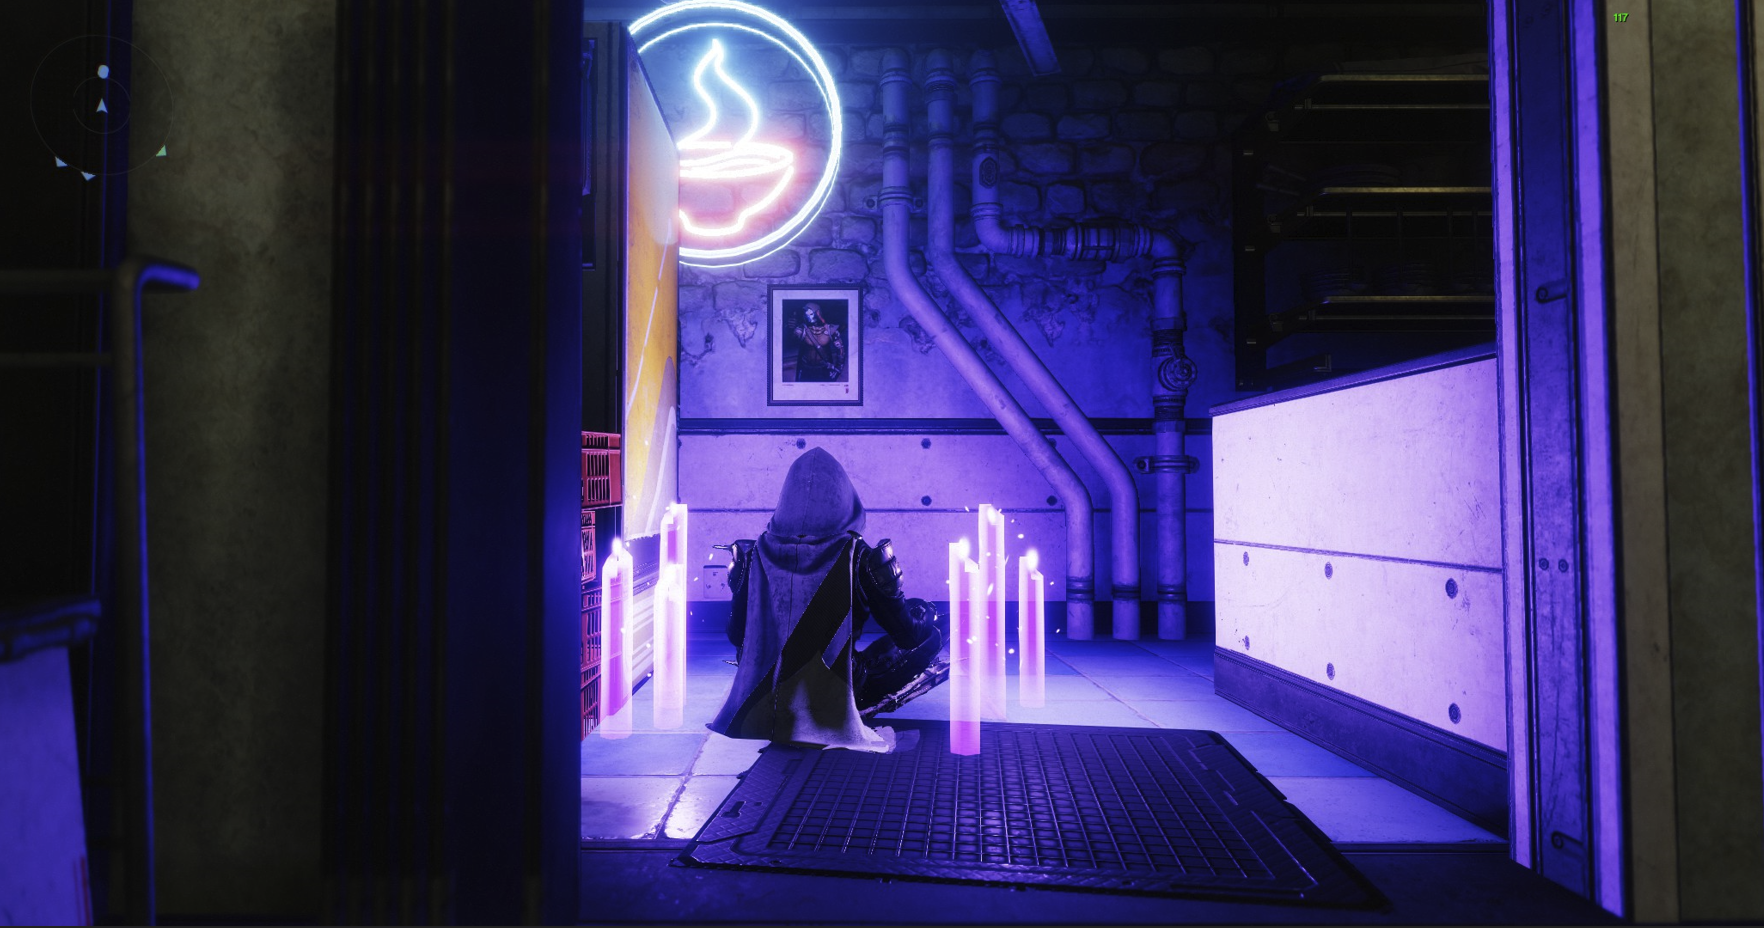
\includegraphics[scale=0.18]{pics/3d_welt_destiny2-environmental-storytelling}
    \caption{Environmental Storytelling - Destiny 2 Cayde}
    \label{fig:3d_environmental_storytelling_destiny2}
\end {figure}


\subsection{City Grid System}\label{subsec:city-grid-system}
Um die Gestaltung der Welt in BeamVR zu erleichtern, wurde ein Grid System verwendet.
Dafür wurde die Stadt in ein Raster aufgeteilt, an welchem sich alle Objekte der Welt auf allen 3 Achsen (x,y,z) orientieren.
~\ref{fig:grid-system-unity}
Unity stellt so ein Grid Snapping System bereits zur Verf\"ugung, daher wurde f\"ur BeamVR am Anfang der
Modellierungsphase eine Bestimmte Grid-Gr\"osse festgelegt, an dem die Grundfl\"achen der Geb\"aude und die Strassen
angepasst wurden.

\begin {figure}
    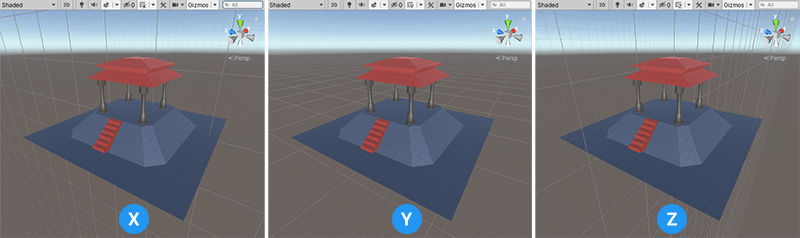
\includegraphics[scale=0.18]{pics/unity-grid-snapping}
    \caption{Unity - Grid Snapping System}
    \label{fig:grid-system-unity}
\end {figure}

Wenn mann die Grid Size, also die Gr\"osse des Rasters, an dem sich alles Orientiert, \"andern m\"ochte muss man zuerst das Grid and Snap Fenster aufrufen.
Als n\"achstes findet man unter dem Bereich World Grid ein Attribut namens Size, wo man die X, Y und Z Achsen frei und unabh\"angig voneinander umskalieren kann.
Wenn man alle Achsen gleichzeitig umstellen m\"ochte, muss man nur auf das Link Icon, welches sich Links neben dem X befindet, dr\"ucken.
Nun werden alle Achsen immer die gleiche Gr\"osse haben.
~\ref{fig:grid-size-unity}
~\cite{Unity_GridSnapping_2022}

\begin {figure}
    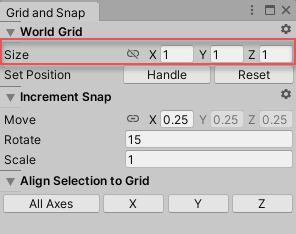
\includegraphics[scale=0.18]{pics/unity-grid-snapping-size}
    \caption{Unity - Grid Snapping Size}
    \label{fig:grid-size-unity}
\end {figure}



\subsection{Stadt}\label{subsec:city}
Jede Stadt hat viele verschiedene Strukturen wie Sehensw\"urdigkeiten, Bauwerke und Einrichtungen wie Kinos, Theater oder Restaurants.
F\"ur BeamVR wurden daher insgesamt \"uber 34 Geb\"aude Modelle erstellt um eine Vielfallt in der Umgebung zu kreieren.
~\ref{fig:beamvr_building-variety}

\begin {figure}
    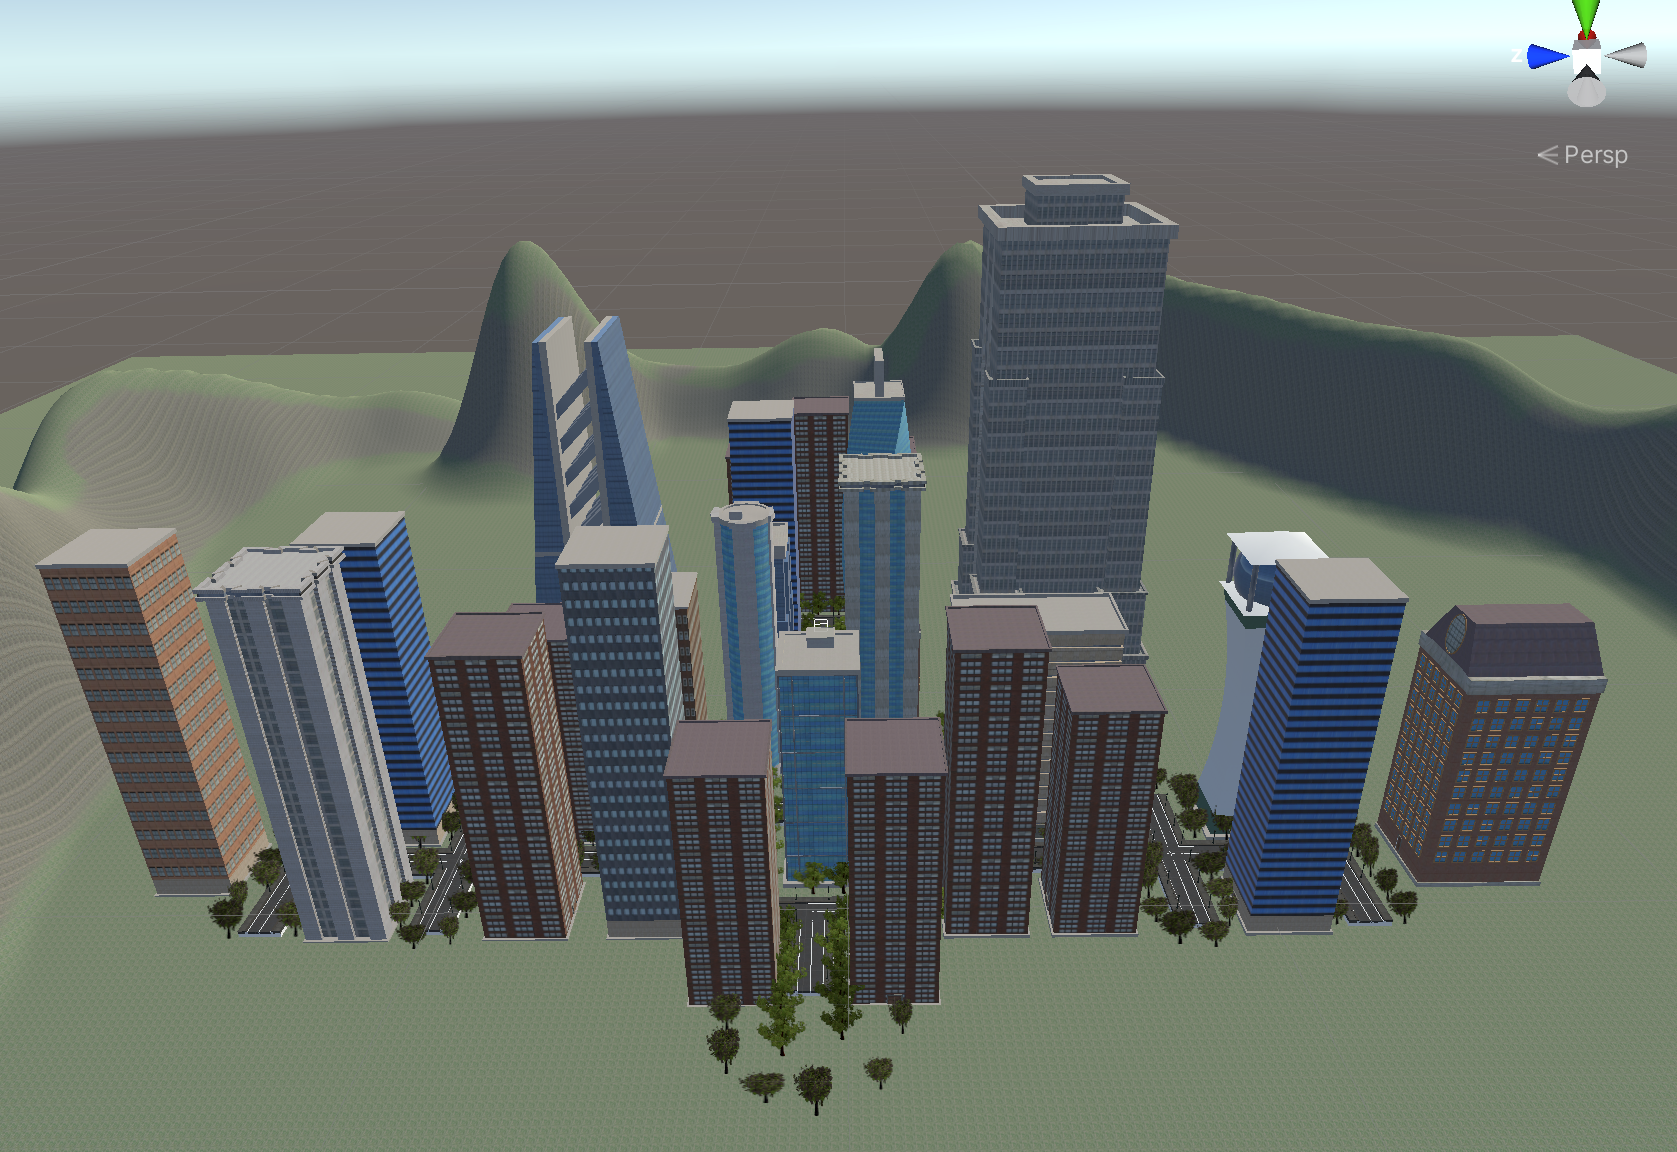
\includegraphics[scale=0.18]{pics/beamvr_building-variety}
    \caption{Beam VR - Building Overview}
    \label{fig:beamvr_building-variety}
\end {figure}

Wie auf dem Bild zu sehen, wurde die Stadt so entworfen, dass nur die für den Spieler sichtbaren Objekte wirklich existieren.
~\ref{fig:beamvr_building-variety}
Bei richtiger Umsetzung scheint es für den Anwender dennoch so, als w\"are dieser in einer kompletten Spielwelt.
In der Spieleentwicklung wird dieser Trick oft angewandt um die Performance des Spieles zu verbessern, da unn\"otige Objekte nicht gerendert oder berechnet werden m\"ussen.
Bei gr\"osseren Projekten spart das nicht nur Zeit sondern auch Ressourcen wie Geld.
Da BeamVR jedoch eine Diplomarbeit ist und daher keine Kosten w\"ahrend der Entwicklung entstehen, wurde dieser Trick angewandt
um die Frames per Second in die h\"ohe zu treiben.


\subsection{Tag Stadt}\label{subsec:day-city}
Es wurden 17 verschieden Geb\"aude f\"ur diese Map modelliert.
~\ref{fig:beamvr_building-variety}
Der Fokus bei der Gestaltung des Bauwerke lag dabei, dass diese m\"oglichst realistisch Aussehen und dennoch nicht zu Rechenaufwendig in der Darstellung werden.
Daher wurden Texturen verwendet um kleinere Details an den Fassaden darzustellen.
Das gleiche wurde bei der Apocalypsen Map angewandt.
~\ref{subsec:apocalypse-city}
Die angewandten Texturen stellen Fassaden aus Stein und Glas dar.
Ein weiterer wichtiger Punkt bei der Planung der Stadt war es auch, dass der Spieler nicht aus der Stadt raus schauen kann.
Daher wurden alle umliegenden Bauwerke mindestens 3 Meter h\"oher gemacht, als das Geb\"aude wo der Spieler steht.
~\ref{fig:beamvr_building-heights}

\begin {figure}
    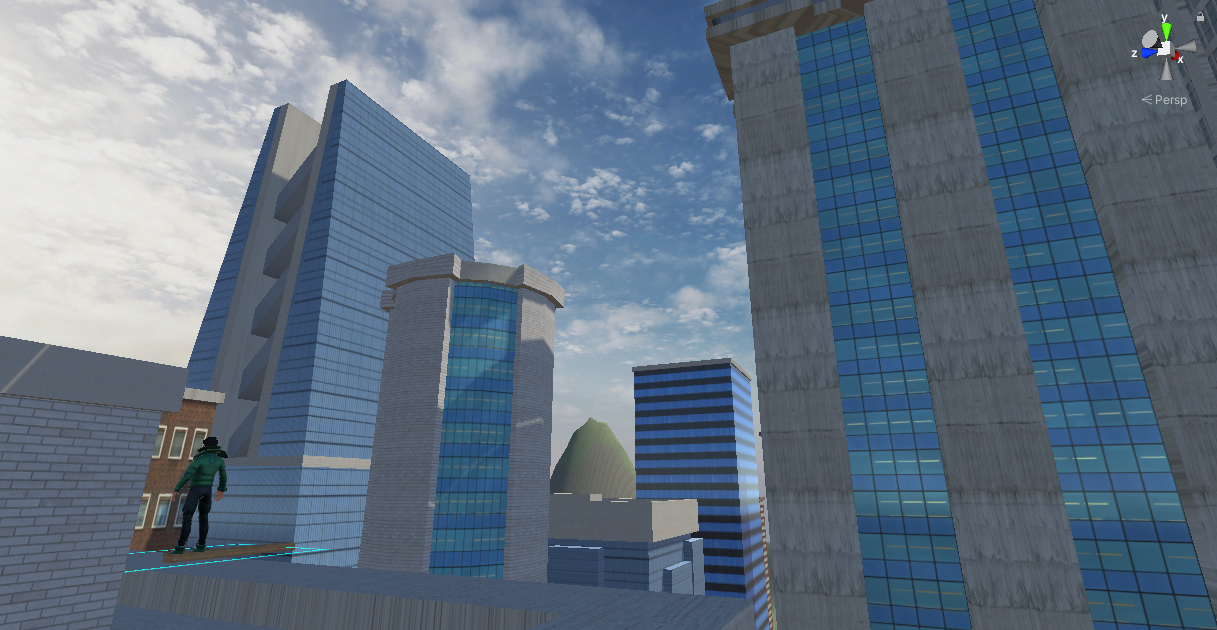
\includegraphics[scale=0.18]{pics/beamvr_city_day_heights}
    \caption{Beam VR - Building Heights}
    \label{fig:beamvr_building-heights}
\end {figure}

\subsection{Nacht Stadt}\label{subsec:night-city}

\subsection{Apokalypsen Stadt}\label{subsec:apocalypse-city}
F\"ur diese Umgebung wurden alle Geb\"aude nochmal \"uberarbeitet.
Statt den intakten Glasfassaden werden nun barrikadierte Fenster und Ziegelsteine ohne Verputz f\"ur die Bauwerke verwendet.
~\ref{fig:beamvr_damaged_texture}
Durch diese \"Anderung sieht die Stadt verlassen und wie nach einer Apokalypse aus.
Um den Effekt noch zus\"atzlich zu verst\"arken wurden die Bauwerke noch etwas verdreht, so dass es aussieht, als w\"urden Diese gleich umkippen.
Das Gel\"ande wurde mit neuen Sandstein Texturen und D\"unen in eine W\"uste umgewandelt.
Die Planzen und B\"aume wurden durch ausgetrocknete B\"usche ausgetauscht, damit die Welt ein trostloses aussehen bekommt.
~\ref{fig:beamvr_apocalypse_map}

\begin {figure}
    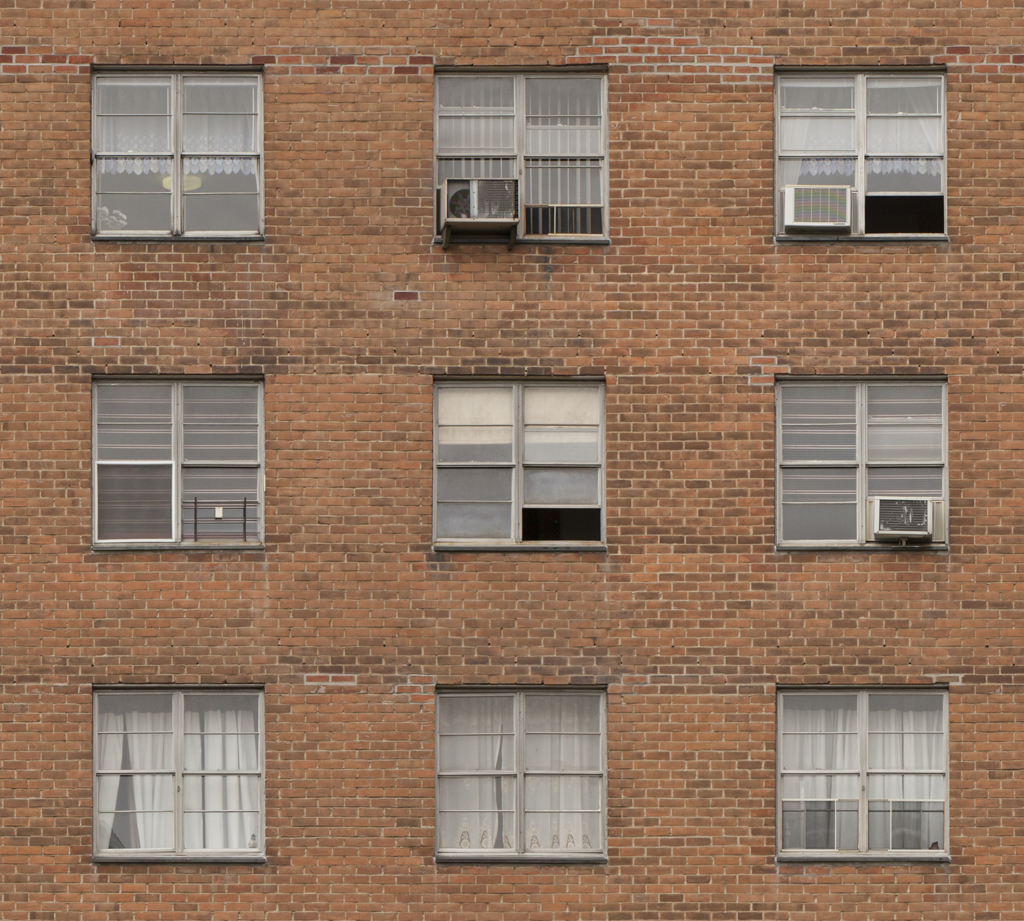
\includegraphics[scale=0.18]{pics/beamvr_damaged_texture}
    \caption{Beam VR - Damaged Texture}
    \label{fig:beamvr_damaged_texture}
\end {figure}

\begin {figure}
    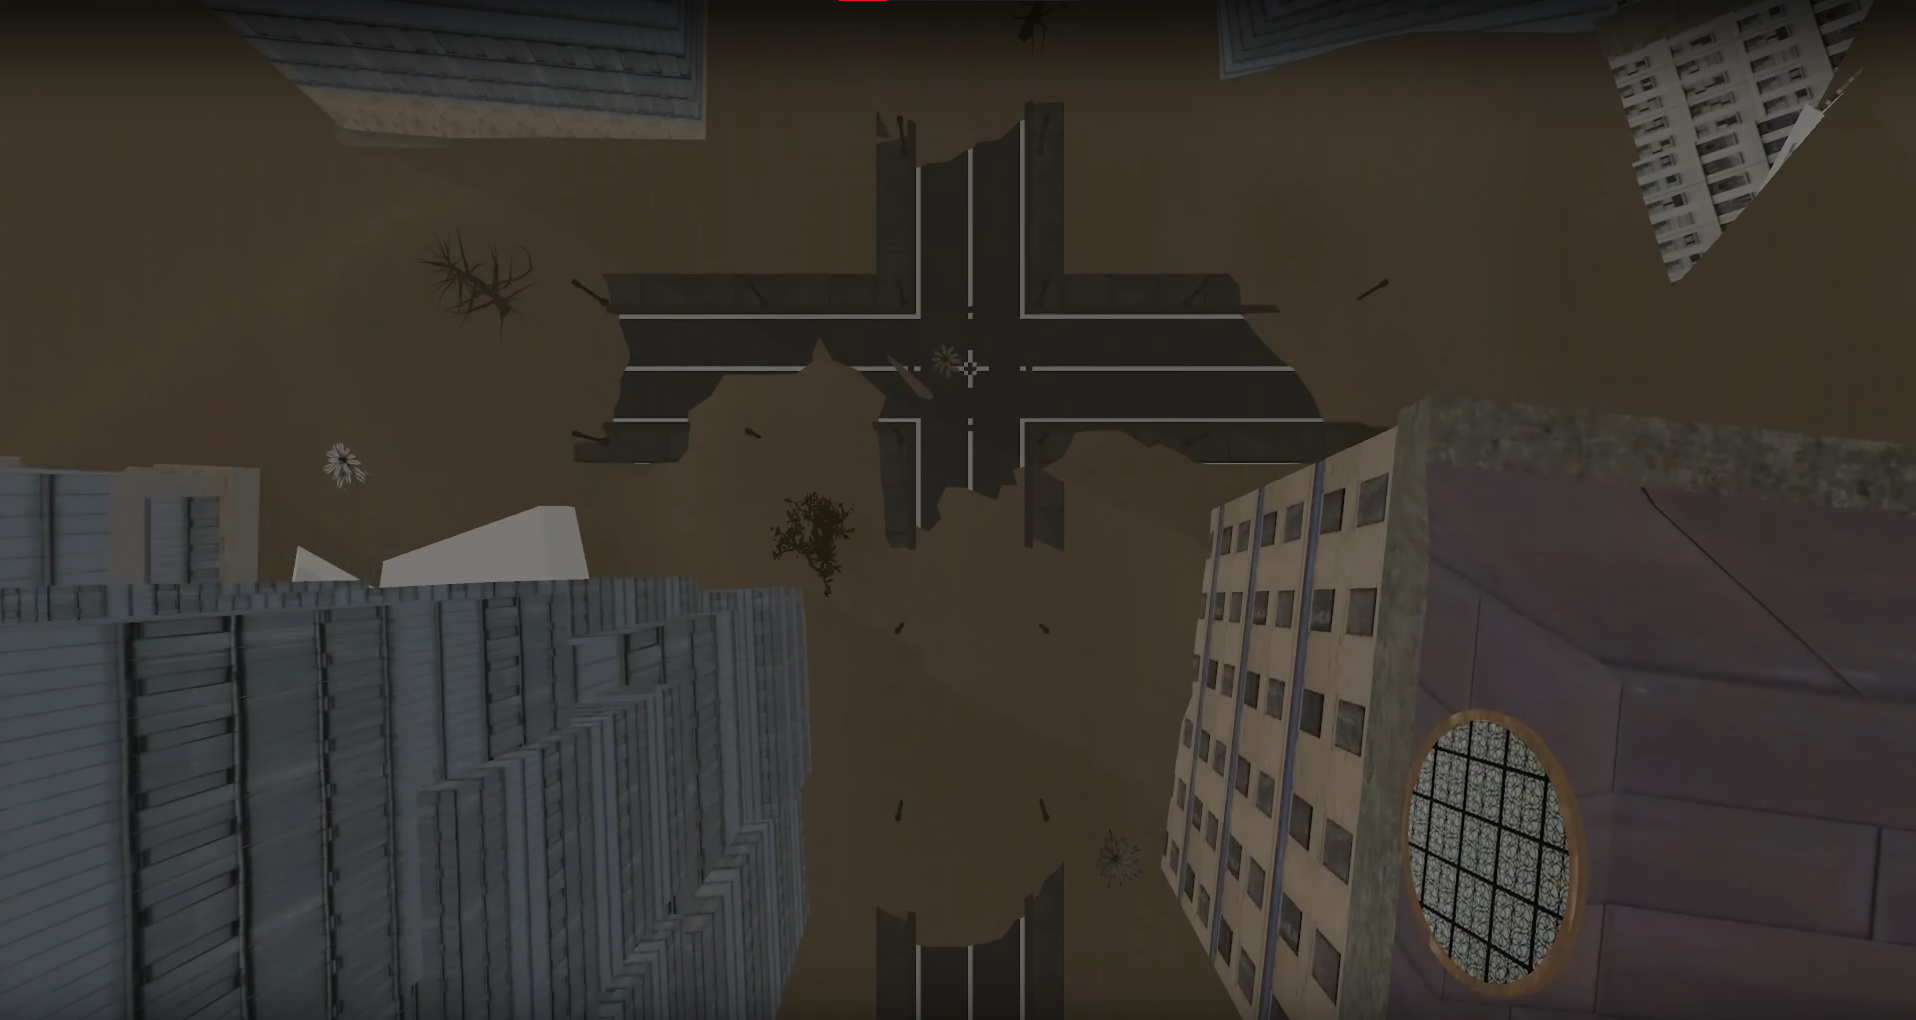
\includegraphics[scale=0.18]{pics/beamvr_apocalypse-overview}
    \caption{Beam VR - Apocalypse Map}
    \label{fig:beamvr_apocalypse_map}
\end {figure}



\section{Sound Design}\label{sec:sound}

\subsection{Apocalypse}\label{subsec:apocalypse-background-sound}

\subsection{City}\label{subsec:day-night-background-sound}

\subsection{Event}\label{subsec:building-collapse-sound}

\section{Effects}\label{sec:effects}

\subsection{Nebel}\label{subsec:fog-effect}

\subsection{Lichter}\label{subsec:light-effect}

\subsection{Wind}\label{subsec:wind-effect}

\section{Unity Prefabs}\label{sec:prefabs}
\subsection{Game}\label{subsec:game-prefab}
\subsection{CameraRigGame}\label{subsec:camera-rig-game-prefab}
\subsection{CameraRigMenu}\label{subsec:camera-rig-menu-prefab}
\section{Inbetriebnahme}\label{sec:commissioning}
